\section{Analysis of the results}
\newcolumntype{C}{>{\Centering\arraybackslash\hspace{0pt}}X}


\pgfplotstableread{
    X Y
    0.7601666451 5
    1.288158894 10
    2.050116062 15
    2.63982296 20
    3.091802597 25
    3.819538355 30
    4.442822933 35
    5.081979036 40
    5.706284046 45
    6.370962858 50
    7.020516396 55
    7.723451853 60
}\vietetable

\pgfplotstableread{
    X Y
    0.5919837952 5
    1.307063103 10
    1.902475357 15
    2.679748535 20
    3.212277889 25
    3.904948235 30
    4.547913074 35
    5.255579948 40
    5.837199688 45
    6.578524113 50
    7.270073891 55
    8.004565239 60

}\madhavatable


\pgfplotstableread{
    X Y
    10  5
    17  10
    27  15
    35  20
    42  25
    51  30
    59  35
    67  40
    76  45
    84  50
    92  55
    101 60
}\vietetableiter

\pgfplotstableread{
    X Y
    9 5
    20 10
    29 15
    41 20
    50 25
    61 30
    71 35
    82 40
    91 45
    102 50
    112 55
    123 60
}\madhavatableiter


\subsection{Presentation of the data}

\subsubsection{Tabular presentation}

The arithmetic mean of a decimal place was calculated for 100 trials and the data points
in the table shown below were found (rounded to 3 significant figures). The values for the decimal place
0 have been dropped as it would not be logical to include them. 

\begin{table}[h]
    \noindent% <-- important
    \setlength\tabcolsep{3pt} % default: 6pt
    \begin{tabularx}{\textwidth}{@{} l *{6}{C} @{}}
        \toprule
        Decimal place & Average time for approximation using Viete's method, in milliseconds (ms) & Average time for approximation using Madhava's method method, in milliseconds (ms) \\
        \midrule
        5             & 0.760                                                                     & 0.592                                                                              \\
        10            & 1.29                                                                      & 1.31                                                                               \\
        15            & 2.05                                                                      & 1.9                                                                                \\
        20            & 2.64                                                                      & 2.68                                                                               \\
        25            & 3.09                                                                      & 3.21                                                                               \\
        30            & 3.82                                                                      & 3.9                                                                                \\
        35            & 4.44                                                                      & 4.55                                                                               \\
        40            & 5.08                                                                      & 5.26                                                                               \\
        45            & 5.71                                                                      & 5.84                                                                               \\
        50            & 6.37                                                                      & 6.58                                                                               \\
        55            & 7.02                                                                      & 7.27                                                                               \\
        60            & 7.72                                                                      & 8.00
    \end{tabularx}
\end{table}

\begin{table}[h]
    \noindent% <-- important
    \setlength\tabcolsep{3pt} % default: 6pt
    \begin{tabularx}{\textwidth}{@{} l *{6}{C} @{}}
        \toprule
        Decimal place & Iterations needed, Viète's method (no unit) & Iterations needed, Madhava's method (no unit) \\
        \midrule
        5             & 10                                          & 9                                             \\
        10            & 17                                          & 20                                            \\
        15            & 27                                          & 29                                            \\
        20            & 35                                          & 41                                            \\
        25            & 42                                          & 50                                            \\
        30            & 51                                          & 61                                            \\
        35            & 59                                          & 71                                            \\
        40            & 67                                          & 82                                            \\
        45            & 76                                          & 91                                            \\
        50            & 84                                          & 102                                           \\
        55            & 92                                          & 112                                           \\
        60            & 101                                         & 123
    \end{tabularx}
\end{table}


The iterations needed for both methods were also measured, using the Python program
(see appendix), slightly modified to increment a variable \verb|i| and subsequently
return it, writing it in a similar manner to a \verb|.csv| file.



\subsubsection{Graphical presentation}

Shown below is a graph demonstrating the correlation between the decimal places approximated
and the amount of iterations needed for this specific decimal milestone. The blue markers and
line of best-fit respresent the results received from Viète's method while the red represent those
from Madhava's method. \\

\begin{tikzpicture}[scale=1.1]
    \begin{axis}[
            title={Comparing the iterations needed for approximating the value of $\pi$},
            xlabel={Iterations},
            ylabel={Decimal places},
            xmin=0, xmax=130,
            ymin=0, ymax=60,
            ytick={0,10,20,30,40,50,60},
            xtick={0,10,20,30,40,50,60,70,80,90,100,110,120,130},
            legend pos=south east,
            ymajorgrids=true,
            grid style=dashed,
            scale=1.2
        ]

        \addplot[
            only marks,
            color=blue,
            mark=*,
        ] table {\vietetableiter};
        \legend{Viète's method}

        \addplot [thin, blue] table[
                y={create col/linear regression={y=Y}}
            ] % compute a linear regression from the input table
            {\vietetableiter};
        \addlegendentry{best fit line}



        \addplot[
            only marks,
            color=red,
            mark=*,
        ] table {\madhavatableiter};
        \addlegendentry{Madhava's method}

        \addplot [thin, red] table[
                y={create col/linear regression={y=Y}}
            ] % compute a linear regression from the input table
            {\madhavatableiter};
        \addlegendentry{best fit line}

    \end{axis}
\end{tikzpicture}

To show the trend in the time data collected, see below the decimal places compared
to the time taken per method. The color coding here is relevant to the one aforementioned. \\

\begin{tikzpicture}[scale=1.1]
    \begin{axis}[
            title={Comparing the time taken for approximating the value of $\pi$},
            xlabel={Time taken [ms]},
            ylabel={Decimal places},
            xmin=0, xmax=10,
            ymin=0, ymax=60,
            ytick={0,10,20,30,40,50,60},
            xtick={0,2,4,6,8,10},
            legend pos=south east,
            ymajorgrids=true,
            grid style=dashed,
            scale=1.2
        ]

        \addplot[
            only marks,
            color=blue,
            mark=*,
        ] table {\vietetable};
        \legend{Viète's method}

        \addplot [thin, blue] table[
                y={create col/linear regression={y=Y}}
            ] % compute a linear regression from the input table
            {\vietetable};
        \addlegendentry{best fit line}



        \addplot[
            only marks,
            color=red,
            mark=*,
        ] table {\madhavatable};
        \addlegendentry{Madhava's method}

        \addplot [thin, red] table[
                y={create col/linear regression={y=Y}}
            ] % compute a linear regression from the input table
            {\madhavatable};
        \addlegendentry{best fit line}

    \end{axis}
\end{tikzpicture}




\subsection{Observations and analysis}

The results gathered from this experiment show linear relationship between the amount of decimal
places approximated and the time required for this approximation, as well as between the decimal places
and the amount of iterations needed. The two lines of best fit for the two methods show
similarities but also differences.

Where decimal places and iterations are compared, there is a clear difference between the two
methods: Madhava's method indeed takes more iterations to converge to a specific decimal of
the value $\pi$. However, in the second graph comparing time, it can be noted that Madhava's
method is marginally faster until the decimal 20, when the lines of the two methods stray apart. It could be
assumed that this occurrence is due to differences between the types of the two methods. Although it 
could be argued that this difference is only due to random error, the results in this graph 
are those collected from the arithmetic mean over 100 trials, and so it can be assessed that this is not the case. Madhava's
method is what is called an alternating series, due to its nature of alternating between values in order
to converge to a specific value, in this case $\pi$, while Viète's method is an infinite product. The
difference between these two methods is underlined in (Figure 3) \ref{fig:comparaison}. It can be
deduced that at lower decimal values Madhava's method is faster as Viète's method's approximation
accuracy firstly increases in what seems similar to a curve from an exponential function $f(x) = k^x$.
It can also be said that while Madhava's method alternates between values such that $m_{n} > \pi, m_{n+1} < \pi$,
Viète's method $\pi_v$ approximates pi in a manner such that $\pi_v < \pi$.

\begin{figure}[h]
    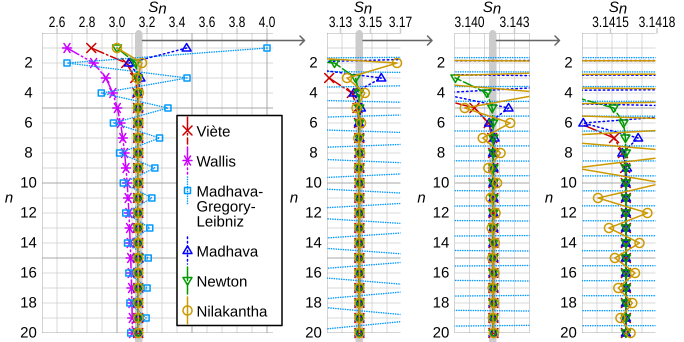
\includegraphics[width=\linewidth]{image.png}
    \caption{Comparison of historical methods of approximating the value of $\pi$. This image demonstrates
        their convergence rates. The line labelled Madhava in dark blue is the method used in this paper.
        From (Wikimedia Commons) \cite{infinite_series_comparaison}}
    \label{fig:comparaison}
\end{figure}
